\documentclass{article}\usepackage[]{graphicx}\usepackage[]{color}
%% maxwidth is the original width if it is less than linewidth
%% otherwise use linewidth (to make sure the graphics do not exceed the margin)
\makeatletter
\def\maxwidth{ %
  \ifdim\Gin@nat@width>\linewidth
    \linewidth
  \else
    \Gin@nat@width
  \fi
}
\makeatother

\definecolor{fgcolor}{rgb}{0.345, 0.345, 0.345}
\newcommand{\hlnum}[1]{\textcolor[rgb]{0.686,0.059,0.569}{#1}}%
\newcommand{\hlstr}[1]{\textcolor[rgb]{0.192,0.494,0.8}{#1}}%
\newcommand{\hlcom}[1]{\textcolor[rgb]{0.678,0.584,0.686}{\textit{#1}}}%
\newcommand{\hlopt}[1]{\textcolor[rgb]{0,0,0}{#1}}%
\newcommand{\hlstd}[1]{\textcolor[rgb]{0.345,0.345,0.345}{#1}}%
\newcommand{\hlkwa}[1]{\textcolor[rgb]{0.161,0.373,0.58}{\textbf{#1}}}%
\newcommand{\hlkwb}[1]{\textcolor[rgb]{0.69,0.353,0.396}{#1}}%
\newcommand{\hlkwc}[1]{\textcolor[rgb]{0.333,0.667,0.333}{#1}}%
\newcommand{\hlkwd}[1]{\textcolor[rgb]{0.737,0.353,0.396}{\textbf{#1}}}%

\usepackage{framed}
\makeatletter
\newenvironment{kframe}{%
 \def\at@end@of@kframe{}%
 \ifinner\ifhmode%
  \def\at@end@of@kframe{\end{minipage}}%
  \begin{minipage}{\columnwidth}%
 \fi\fi%
 \def\FrameCommand##1{\hskip\@totalleftmargin \hskip-\fboxsep
 \colorbox{shadecolor}{##1}\hskip-\fboxsep
     % There is no \\@totalrightmargin, so:
     \hskip-\linewidth \hskip-\@totalleftmargin \hskip\columnwidth}%
 \MakeFramed {\advance\hsize-\width
   \@totalleftmargin\z@ \linewidth\hsize
   \@setminipage}}%
 {\par\unskip\endMakeFramed%
 \at@end@of@kframe}
\makeatother

\definecolor{shadecolor}{rgb}{.97, .97, .97}
\definecolor{messagecolor}{rgb}{0, 0, 0}
\definecolor{warningcolor}{rgb}{1, 0, 1}
\definecolor{errorcolor}{rgb}{1, 0, 0}
\newenvironment{knitrout}{}{} % an empty environment to be redefined in TeX

\usepackage{alltt}
\usepackage{fullpage}
\usepackage[colorlinks=true,linkcolor=blue]{hyperref}

\title{STAT 675 Homework \# 3}
\author{Dominic D LaRoche}
\IfFileExists{upquote.sty}{\usepackage{upquote}}{}
\begin{document}
\begin{itemize}
\item[7.1]  Jackknife estimate of the bias and standard error of the correlation statistic.\\

\begin{knitrout}
\definecolor{shadecolor}{rgb}{0.969, 0.969, 0.969}\color{fgcolor}\begin{kframe}
\begin{alltt}
\hlkwd{require}(bootstrap)
\hlkwd{require}(boot)
\hlkwd{data}(law)
n <- \hlkwd{dim}(law)[1]
rho <- \hlkwd{cor}(law$LSAT, law$GPA)
rho.jack <- \hlkwd{numeric}(n)
\hlkwd{for} (i in 1:n) \{
    rho.jack[i] <- \hlkwd{cor}(law$LSAT[-i], law$GPA[-i])
\}
bias <- (n - 1) * (\hlkwd{mean}(rho.jack) - rho)
rho.mean <- \hlkwd{mean}(rho.jack)
se <- \hlkwd{sqrt}((n - 1) * \hlkwd{mean}((rho.jack - rho.mean)^2))
\end{alltt}
\end{kframe}
\end{knitrout}

The bias is calculated as -0.0065 and the standard error is calculated as 0.1425.\\

\item[7.4]  The pdf of the exponential distribution is $f(x)= \lambda e^{-\lambda x} I_{(0,\inf)}(X)$.  The maximum likelihood estimator $\hat{\lambda}$ is:\\
$$L(\lambda|x)=\prod_{i=1}^n \lambda e^{-\lambda x_i} I_{(0,\inf)}(x_i)= \lambda^n e^{-\lambda \sum x_i} I_{(0,\inf)}(x_i)$$
$$log(L(\lambda|x)) = l = n log(\lambda)-\lambda \sum x_i$$
$$l^{\prime}= \frac{n}{\lambda}-\sum x_i$$
$$\frac{n}{\hat{\lambda}} = \sum x_i$$
$$\hat{\lambda}= \frac{n}{\sum x_i} = \frac{1}{\bar{x}}$$

\begin{knitrout}
\definecolor{shadecolor}{rgb}{0.969, 0.969, 0.969}\color{fgcolor}\begin{kframe}
\begin{alltt}
\hlkwd{set.seed}(36)
\hlkwd{data}(aircondit)
air <- aircondit  \hlcom{#shorten the name for easier coding}
lambda <- 1/\hlkwd{mean}(air$hours)
r <- 10000
\hlkwd{set.seed}(36)
lambda.boot <- \hlkwd{boot}(data = air, statistic = \hlkwd{function}(x, i) \{
    1/\hlkwd{mean}(x[i, ])
\}, R = r)
lambda.boot
\end{alltt}
\begin{verbatim}
## 
## ORDINARY NONPARAMETRIC BOOTSTRAP
## 
## 
## Call:
## boot(data = air, statistic = function(x, i) {
##     1/mean(x[i, ])
## }, R = r)
## 
## 
## Bootstrap Statistics :
##     original   bias    std. error
## t1* 0.009252 0.001406    0.004397
\end{verbatim}
\end{kframe}
\end{knitrout}


\item[7.5] Bootstrap confidence intervals via standard normal, basic, percentile, and BCa methods.\\
From the invariance property of the MLE, $\frac{1}{\hat{\lambda}}=\bar{x}$ is a function of a MLE estimator and is therefore also a MLE estimator.\\  
The standard normal CI is calculated without bootstraping:\\
\begin{knitrout}
\definecolor{shadecolor}{rgb}{0.969, 0.969, 0.969}\color{fgcolor}\begin{kframe}
\begin{alltt}
mtime <- \hlkwd{mean}(air$hours)
se.norm <- \hlkwd{sd}(air$hours)/\hlkwd{sqrt}(\hlkwd{dim}(air)[1])
mtime.CI <- \hlkwd{c}(mtime - (1.96 * se.norm), mtime, mtime + (1.96 * se.norm))
mtime.CI
\end{alltt}
\begin{verbatim}
## [1]  31.0 108.1 185.2
\end{verbatim}
\end{kframe}
\end{knitrout}

The bootstrap confidence intervals are:
\begin{knitrout}
\definecolor{shadecolor}{rgb}{0.969, 0.969, 0.969}\color{fgcolor}\begin{kframe}
\begin{alltt}
\hlkwd{set.seed}(36)
mtime.boot <- \hlkwd{boot}(data = air, statistic = \hlkwd{function}(x, i) \{
    \hlkwd{mean}(x[i, ])
\}, R = r)
einf.jack <- \hlkwd{empinf}(mtime.boot, type = \hlstr{"jack"})
\hlkwd{boot.ci}(mtime.boot, type = \hlkwd{c}(\hlstr{"basic"}, \hlstr{"perc"}, \hlstr{"bca"}), L = einf.jack)
\end{alltt}
\begin{verbatim}
## BOOTSTRAP CONFIDENCE INTERVAL CALCULATIONS
## Based on 10000 bootstrap replicates
## 
## CALL : 
## boot.ci(boot.out = mtime.boot, type = c("basic", "perc", "bca"), 
##     L = einf.jack)
## 
## Intervals : 
## Level      Basic              Percentile            BCa          
## 95%   ( 24.3, 169.8 )   ( 46.3, 191.8 )   ( 56.9, 226.2 )  
## Calculations and Intervals on Original Scale
\end{verbatim}
\end{kframe}
\end{knitrout}

All of these CI's differ substantially.  This is likely because the distribution of the mean interval time is not normal.  To check this we can examine the distribution:
\begin{knitrout}
\definecolor{shadecolor}{rgb}{0.969, 0.969, 0.969}\color{fgcolor}\begin{kframe}
\begin{alltt}
\hlkwd{hist}(mtime.boot$t, main = NULL)
\end{alltt}
\end{kframe}
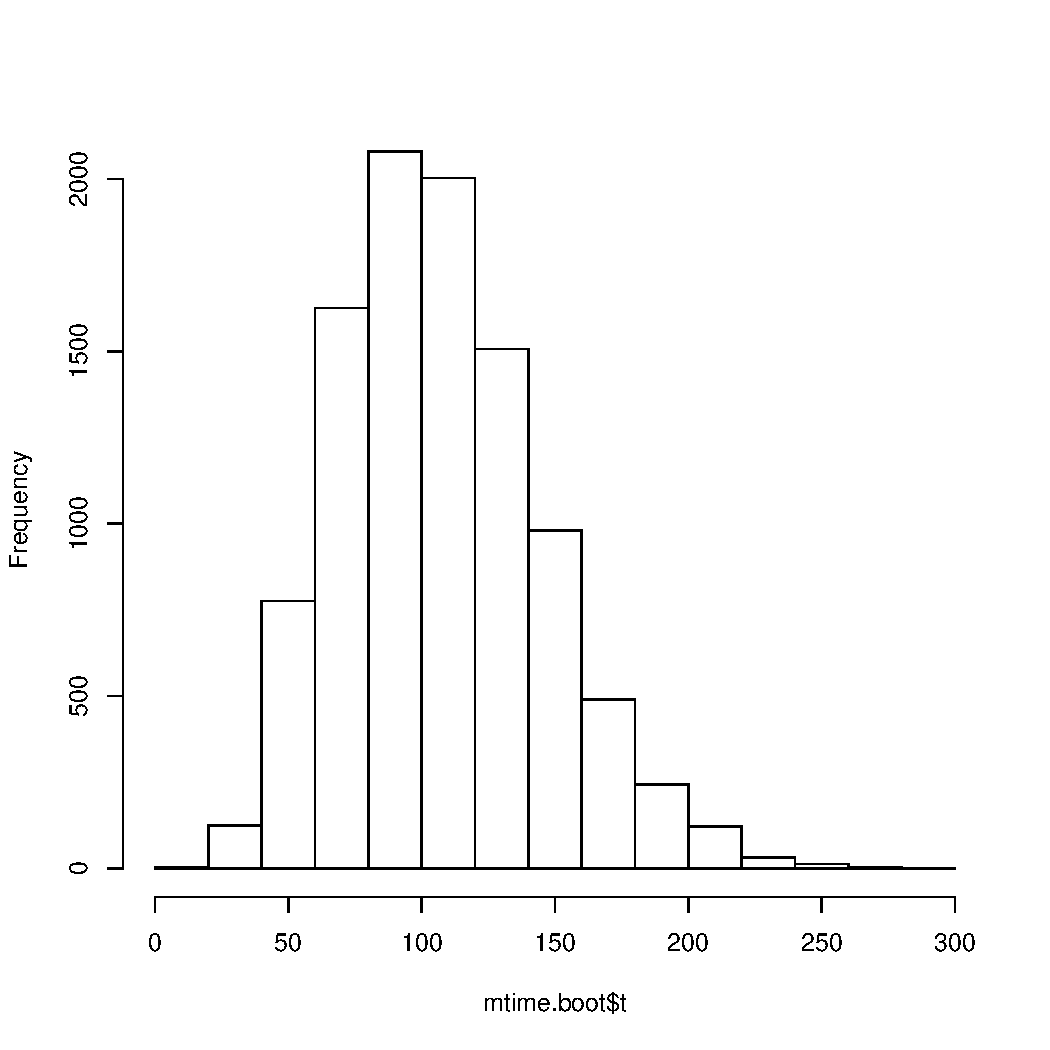
\includegraphics[width=\maxwidth]{figure/sevenc} 

\end{knitrout}

Indeed the distribution has a clear right skew.  The standard normal confidence interval assumes a symmetric normal distribution which is clearly violated in this case.  The basic and percentile methods also assume a symmetric distribution and therefore the BCa method, which accounts for skew, is proabably the best in this case.\\

\item[7.6]  Test data correlations.\\

\begin{knitrout}
\definecolor{shadecolor}{rgb}{0.969, 0.969, 0.969}\color{fgcolor}\begin{kframe}
\begin{alltt}
\hlkwd{data}(scor)
\hlkwd{pairs}(scor)
\end{alltt}
\end{kframe}
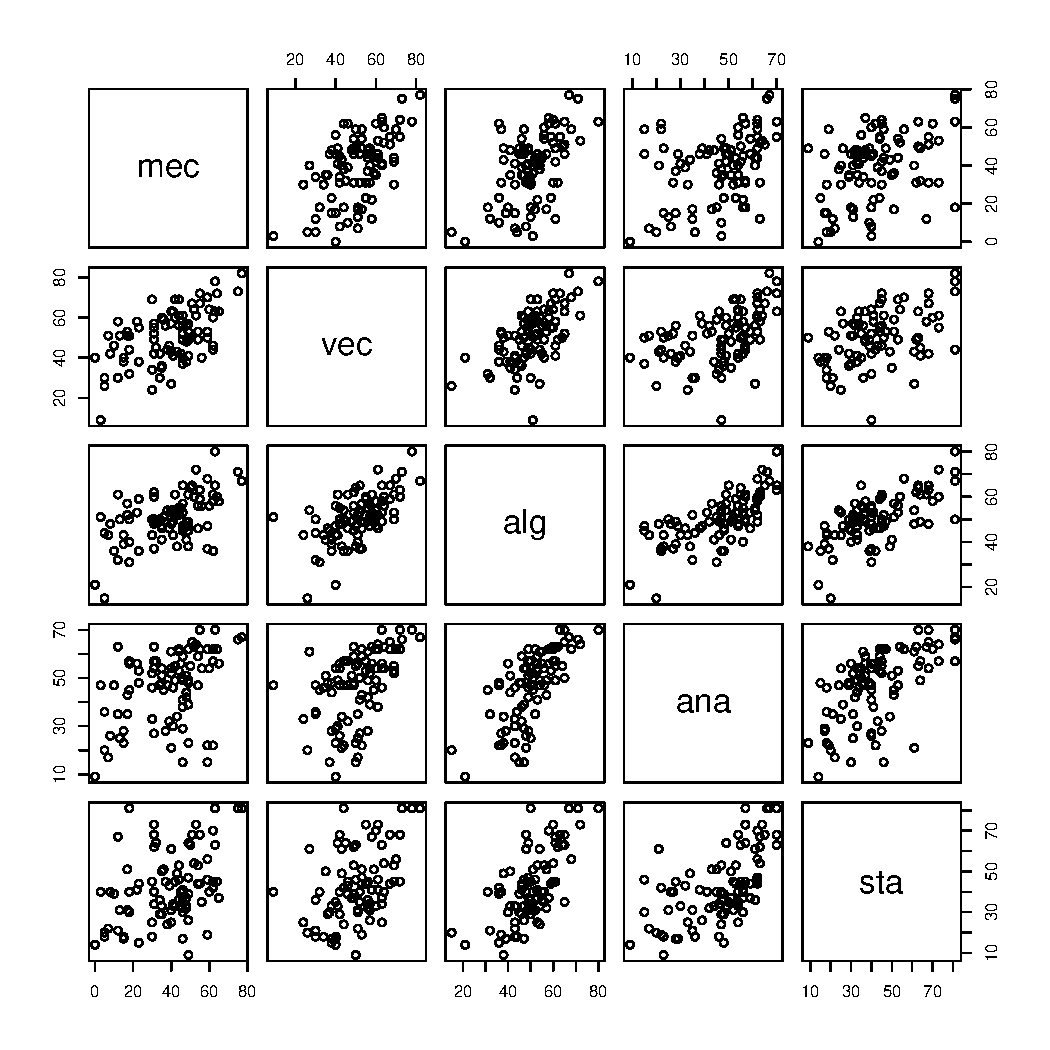
\includegraphics[width=\maxwidth]{figure/seven6} 

\end{knitrout}


The sample correlation matrix contains the same information:\\
\begin{knitrout}
\definecolor{shadecolor}{rgb}{0.969, 0.969, 0.969}\color{fgcolor}\begin{kframe}
\begin{alltt}
\hlkwd{cor}(scor)
\end{alltt}
\begin{verbatim}
##        mec    vec    alg    ana    sta
## mec 1.0000 0.5534 0.5468 0.4094 0.3891
## vec 0.5534 1.0000 0.6096 0.4851 0.4364
## alg 0.5468 0.6096 1.0000 0.7108 0.6647
## ana 0.4094 0.4851 0.7108 1.0000 0.6072
## sta 0.3891 0.4364 0.6647 0.6072 1.0000
\end{verbatim}
\end{kframe}
\end{knitrout}

All of the variables have reasonably strong correlations.  The bootstrap estimates of the standard errors
\begin{knitrout}
\definecolor{shadecolor}{rgb}{0.969, 0.969, 0.969}\color{fgcolor}\begin{kframe}
\begin{alltt}
\hlkwd{set.seed}(36)
corSE.boot <- \hlkwd{function}(var1, var2, rep = 10000) \{
\hlcom{    #function to compute the se of a correlation}
    dat <- \hlkwd{cbind}(var1, var2)
    r <- \hlkwd{function}(dat, i) \{
        \hlkwd{cor}(dat[i, 1], dat[i, 2])
    \}
    dat <- \hlkwd{cbind}(var1, var2)
    obj <- \hlkwd{boot}(data = dat, statistic = r, R = rep)
    y <- obj$t
    \hlkwd{return}(\hlkwd{apply}(y, 2, sd))
\}
\hlkwd{corSE.boot}(scor$mec, scor$vec)
\end{alltt}
\begin{verbatim}
## [1] 0.07602
\end{verbatim}
\begin{alltt}
\hlkwd{corSE.boot}(scor$alg, scor$ana)
\end{alltt}
\begin{verbatim}
## [1] 0.04899
\end{verbatim}
\begin{alltt}
\hlkwd{corSE.boot}(scor$alg, scor$sta)
\end{alltt}
\begin{verbatim}
## [1] 0.06015
\end{verbatim}
\begin{alltt}
\hlkwd{corSE.boot}(scor$ana, scor$sta)
\end{alltt}
\begin{verbatim}
## [1] 0.06752
\end{verbatim}
\end{kframe}
\end{knitrout}


\item[7.7] Bootstrap estimate of the bias and standard error of the estimate of the proportion of variance included in the first PCA component.\\
\begin{knitrout}
\definecolor{shadecolor}{rgb}{0.969, 0.969, 0.969}\color{fgcolor}\begin{kframe}
\begin{alltt}
\hlkwd{set.seed}(36)
l <- \hlkwd{eigen}(\hlkwd{cov}(scor))$values
theta <- l[1]/\hlkwd{sum}(l)
thetafun <- \hlkwd{function}(x, i) \{
    l <- \hlkwd{eigen}(\hlkwd{cov}(x[i, ]))$values
    theta <- l[1]/\hlkwd{sum}(l)
    \hlkwd{return}(theta)
\}
theta.boot <- \hlkwd{boot}(data = scor, statistic = thetafun, R = r)
theta.boot
\end{alltt}
\begin{verbatim}
## 
## ORDINARY NONPARAMETRIC BOOTSTRAP
## 
## 
## Call:
## boot(data = scor, statistic = thetafun, R = r)
## 
## 
## Bootstrap Statistics :
##     original   bias    std. error
## t1*   0.6191 0.000862     0.04808
\end{verbatim}
\end{kframe}
\end{knitrout}


\item[7.8] Jackknife estimate of the bias and standard error of the estimate of the proportion of variance included in the first PCA component.\\
\begin{knitrout}
\definecolor{shadecolor}{rgb}{0.969, 0.969, 0.969}\color{fgcolor}\begin{kframe}
\begin{alltt}
theta.jack <- \hlkwd{numeric}(\hlkwd{dim}(scor)[1])
\hlkwd{for} (i in 1:\hlkwd{length}(theta.jack)) \{
    theta.jack[i] <- \hlkwd{eigen}(\hlkwd{cov}(scor[-i, ]))$values[1]/\hlkwd{sum}(\hlkwd{eigen}(\hlkwd{cov}(scor[-i, 
        ]))$values)
\}
bias <- (\hlkwd{length}(theta.jack) - 1) * (\hlkwd{mean}(theta.jack) - theta)
theta.mean <- \hlkwd{mean}(theta.jack)
se <- \hlkwd{sqrt}((\hlkwd{length}(theta.jack) - 1) * \hlkwd{mean}((theta.jack - theta.mean)^2))
bias
\end{alltt}
\begin{verbatim}
## [1] 0.001069
\end{verbatim}
\begin{alltt}
se
\end{alltt}
\begin{verbatim}
## [1] 0.04955
\end{verbatim}
\end{kframe}
\end{knitrout}


\item[7.9] 95\% percentile and BCa confidence intervals for $\hat{\theta}$.\\
\begin{knitrout}
\definecolor{shadecolor}{rgb}{0.969, 0.969, 0.969}\color{fgcolor}\begin{kframe}
\begin{alltt}
\hlkwd{set.seed}(36)
\hlkwd{boot.ci}(theta.boot, type = \hlkwd{c}(\hlstr{"perc"}, \hlstr{"bca"}), L = \hlkwd{empinf}(theta.boot, type = \hlstr{"jack"}))
\end{alltt}
\begin{verbatim}
## BOOTSTRAP CONFIDENCE INTERVAL CALCULATIONS
## Based on 10000 bootstrap replicates
## 
## CALL : 
## boot.ci(boot.out = theta.boot, type = c("perc", "bca"), L = empinf(theta.boot, 
##     type = "jack"))
## 
## Intervals : 
## Level     Percentile            BCa          
## 95%   ( 0.5200,  0.7090 )   ( 0.5179,  0.7074 )  
## Calculations and Intervals on Original Scale
\end{verbatim}
\end{kframe}
\end{knitrout}


\item[7.10] Model selection via cross-validation.\\
Using code from the book's website
\begin{knitrout}
\definecolor{shadecolor}{rgb}{0.969, 0.969, 0.969}\color{fgcolor}\begin{kframe}
\begin{alltt}
\hlkwd{library}(DAAG)
\end{alltt}


{\ttfamily\noindent\itshape\color{messagecolor}{\#\# Loading required package: lattice\\\#\# \\\#\# Attaching package: 'lattice'\\\#\# \\\#\# The following object(s) are masked from 'package:boot':\\\#\# \\\#\#\ \ \ \  melanoma}}\begin{alltt}
\hlkwd{attach}(ironslag)
a <- \hlkwd{seq}(-12, 12, 0.1)  \hlcom{#sequence for plotting fits}
mchem <- \hlkwd{mean}(chemical)
chem <- chemical - mchem
ironslag$chem <- chem  \hlcom{# center the chemical variable}

L1 <- \hlkwd{lm}(magnetic ~ chem)
\hlkwd{plot}(chem, magnetic, main = \hlstr{"Linear"}, pch = 16)
yhat1 <- L1$coef[1] + L1$coef[2] * a
\hlkwd{lines}(a, yhat1, lwd = 2)
\end{alltt}
\end{kframe}
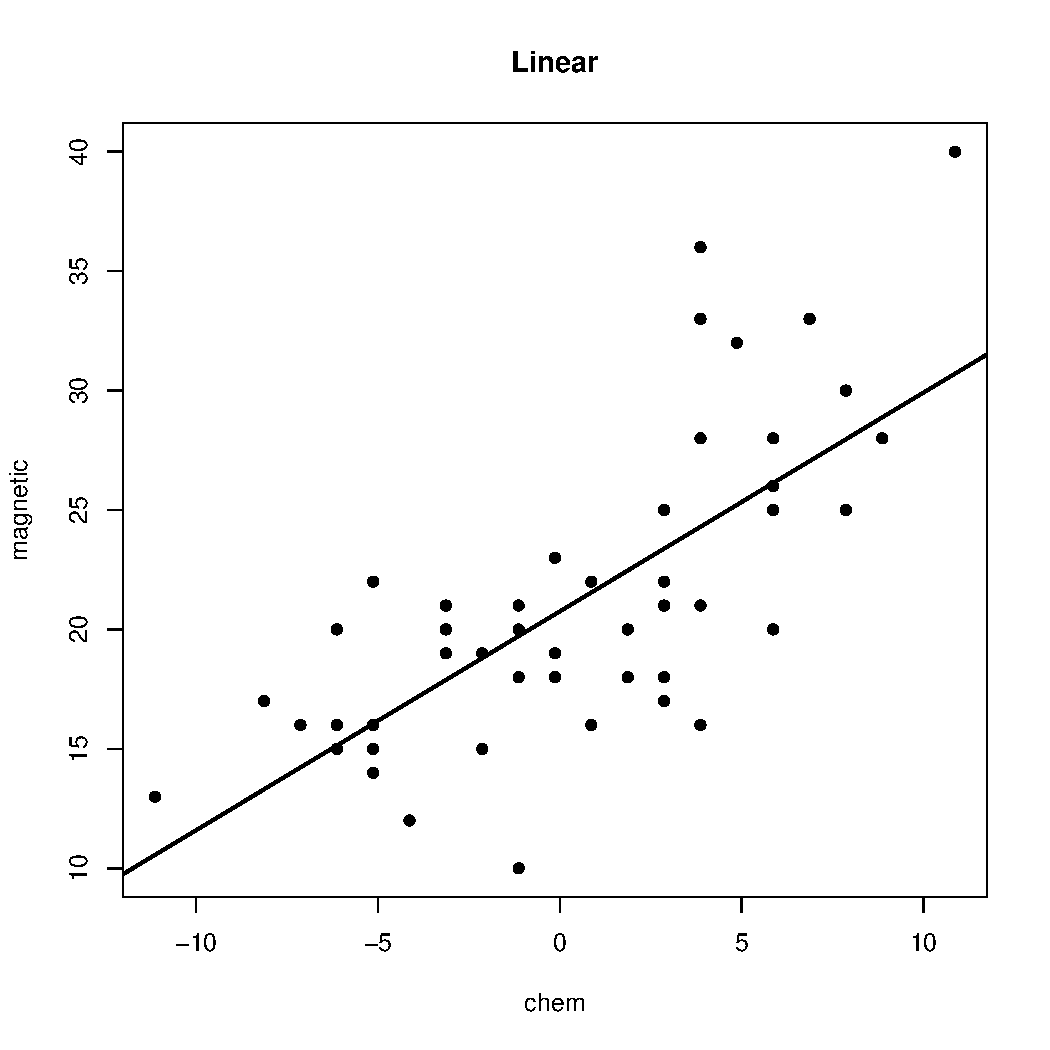
\includegraphics[width=\maxwidth]{figure/seven101} 
\begin{kframe}\begin{alltt}

L2 <- \hlkwd{lm}(magnetic ~ chem + \hlkwd{I}(chem^2))
\hlkwd{plot}(chem, magnetic, main = \hlstr{"Quadratic"}, pch = 16)
yhat2 <- L2$coef[1] + L2$coef[2] * a + L2$coef[3] * a^2
\hlkwd{lines}(a, yhat2, lwd = 2)
\end{alltt}
\end{kframe}
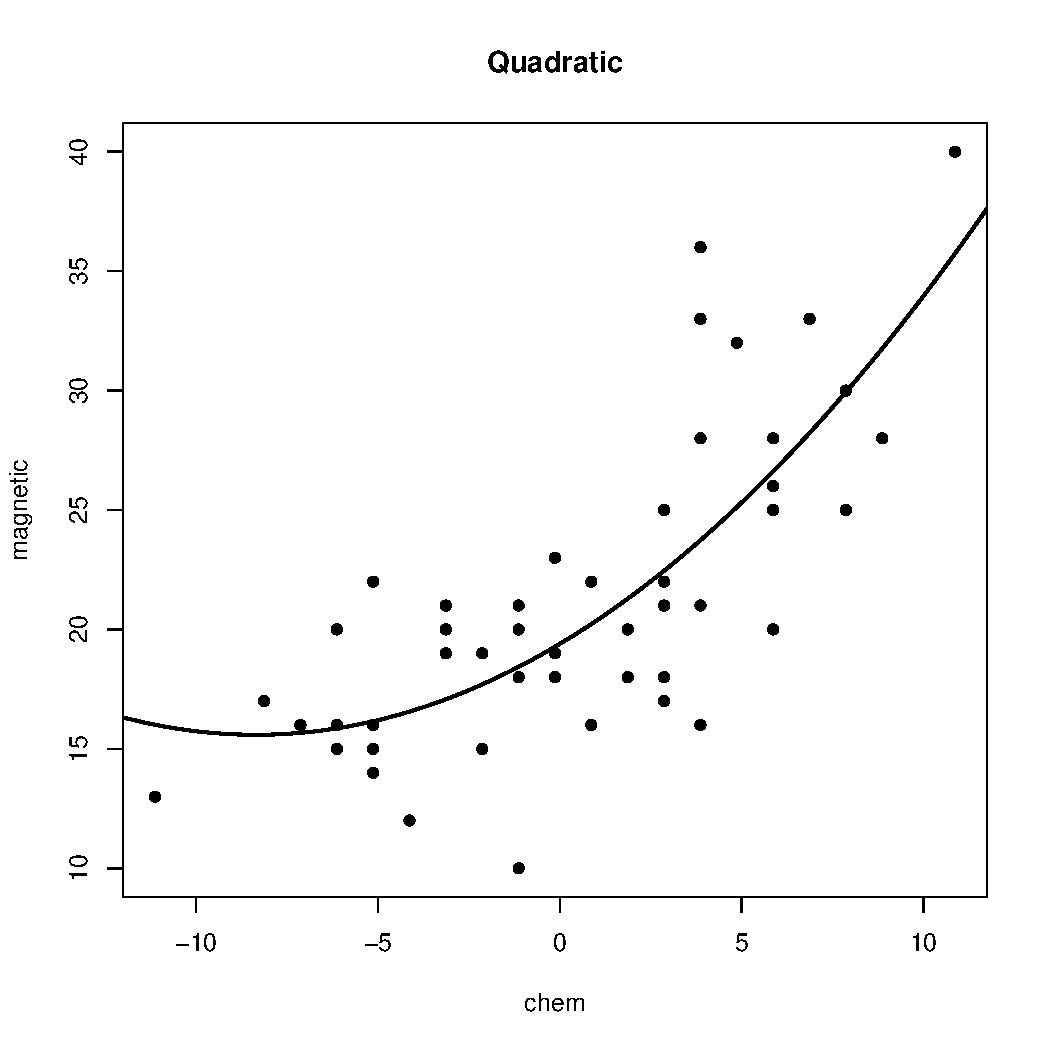
\includegraphics[width=\maxwidth]{figure/seven102} 
\begin{kframe}\begin{alltt}

L3 <- \hlkwd{lm}(\hlkwd{log}(magnetic) ~ chem)
\hlkwd{plot}(chem, magnetic, main = \hlstr{"Exponential"}, pch = 16)
logyhat3 <- L3$coef[1] + L3$coef[2] * a
yhat3 <- \hlkwd{exp}(logyhat3)
\hlkwd{lines}(a, yhat3, lwd = 2)
\end{alltt}
\end{kframe}
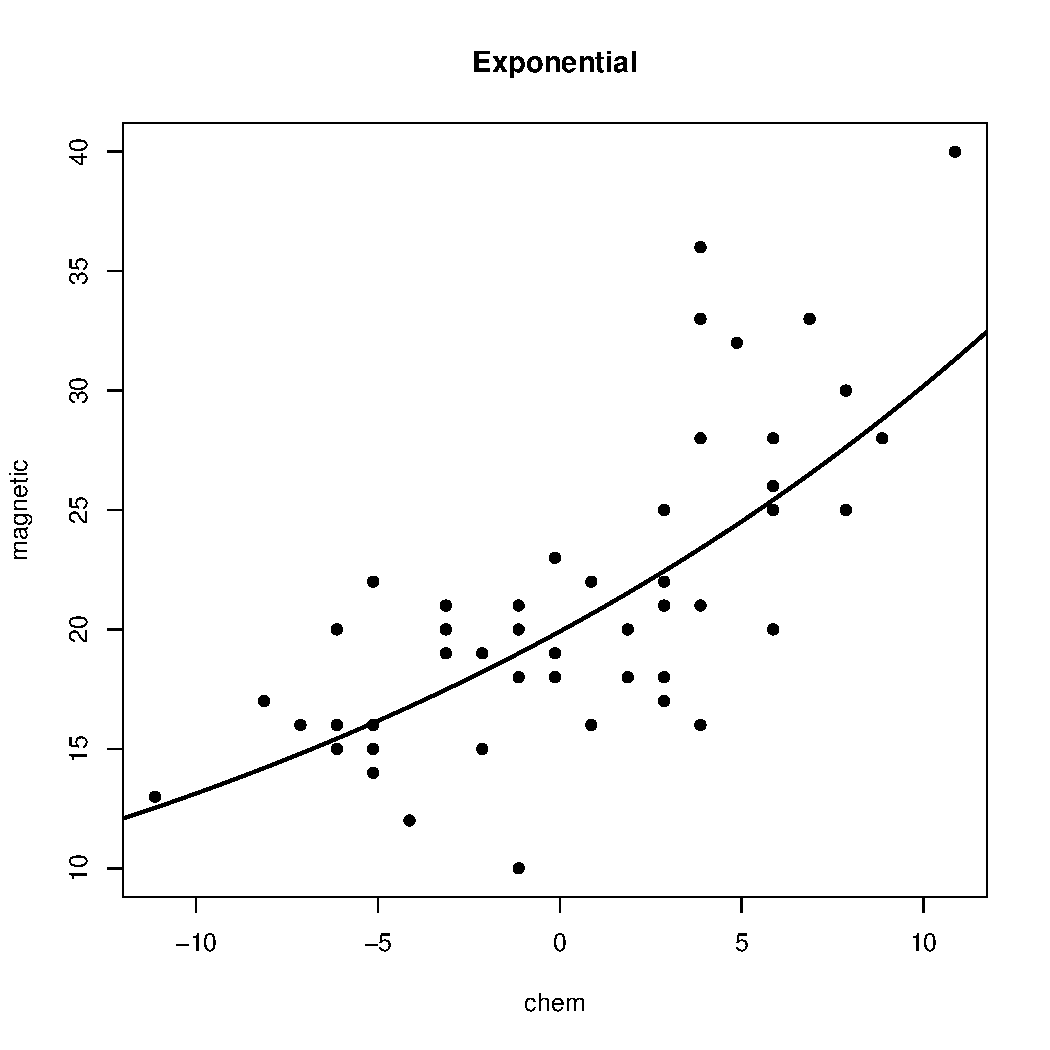
\includegraphics[width=\maxwidth]{figure/seven103} 
\begin{kframe}\begin{alltt}

L4 <- \hlkwd{lm}(magnetic ~ chem + \hlkwd{I}(chem^2) + \hlkwd{I}(chem^3))
\hlkwd{plot}(chem, magnetic, main = \hlstr{"Cubic"}, pch = 16)
yhat4 <- L4$coef[1] + L4$coef[2] * a + L4$coef[3] * a^2 + L4$coef[4] * a^3
\hlkwd{lines}(a, yhat4, lwd = 2)
\end{alltt}
\end{kframe}
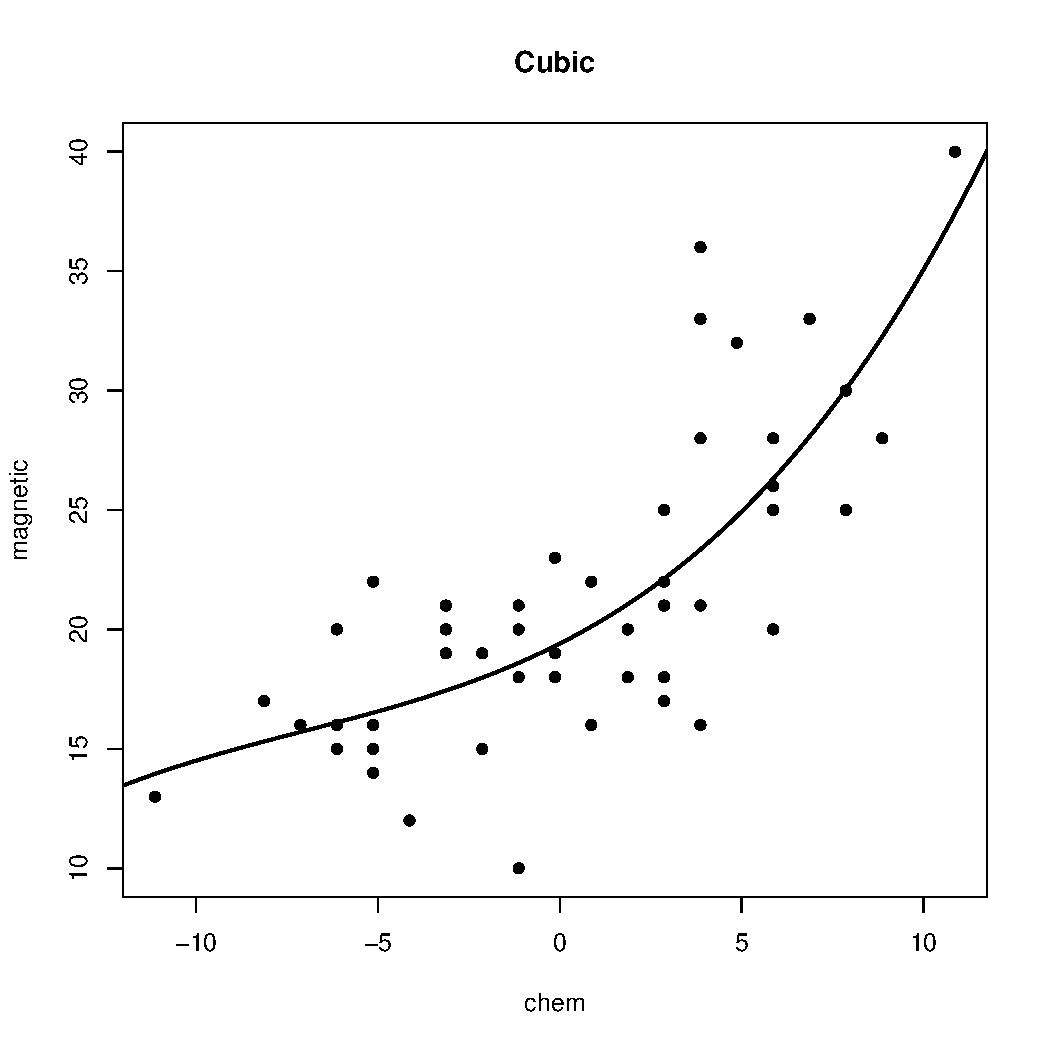
\includegraphics[width=\maxwidth]{figure/seven104} 
\begin{kframe}\begin{alltt}

n <- \hlkwd{length}(magnetic)  \hlcom{#in DAAG ironslag}
e1 <- e2 <- e3 <- e4 <- \hlkwd{numeric}(n)
\hlcom{# for n-fold cross validation fit models on leave-one-out samples}
\hlkwd{for} (k in 1:n) \{
    y <- magnetic[-k]
    x <- chem[-k]
    
    J1 <- \hlkwd{lm}(y ~ x)
    yhat1 <- J1$coef[1] + J1$coef[2] * chem[k]
    e1[k] <- magnetic[k] - yhat1
    
    J2 <- \hlkwd{lm}(y ~ x + \hlkwd{I}(x^2))
    yhat2 <- J2$coef[1] + J2$coef[2] * chem[k] + J2$coef[3] * chem[k]^2
    e2[k] <- magnetic[k] - yhat2
    
    J3 <- \hlkwd{lm}(\hlkwd{log}(y) ~ x)
    logyhat3 <- J3$coef[1] + J3$coef[2] * chem[k]
    yhat3 <- \hlkwd{exp}(logyhat3)
    e3[k] <- magnetic[k] - yhat3
    
    J4 <- \hlkwd{lm}(y ~ x + \hlkwd{I}(x^2) + \hlkwd{I}(x^3))
    yhat4 <- J4$coef[1] + J4$coef[2] * chem[k] + J4$coef[3] * chem[k]^2 + J4$coef[4] * 
        chem[k]^3
    e4[k] <- magnetic[k] - yhat4
\}

mean.error <- \hlkwd{c}(\hlkwd{mean}(e1^2), \hlkwd{mean}(e2^2), \hlkwd{mean}(e3^2), \hlkwd{mean}(e4^2))
mean.error
\end{alltt}
\begin{verbatim}
## [1] 19.56 17.85 18.44 18.18
\end{verbatim}
\begin{alltt}
\hlkwd{which.min}(mean.error)  \hlcom{#The smallest mean error}
\end{alltt}
\begin{verbatim}
## [1] 2
\end{verbatim}
\begin{alltt}

R_squared <- \hlkwd{c}(\hlkwd{summary}(L1)$adj.r.squared, \hlkwd{summary}(L2)$adj.r.squared, \hlkwd{summary}(L3)$adj.r.squared, 
    \hlkwd{summary}(L4)$adj.r.squared)
R_squared
\end{alltt}
\begin{verbatim}
## [1] 0.5282 0.5768 0.5281 0.5740
\end{verbatim}
\begin{alltt}
\hlkwd{which.max}(R_squared)
\end{alltt}
\begin{verbatim}
## [1] 2
\end{verbatim}
\end{kframe}
\end{knitrout}

The adjusted $R^2$ follows the same pattern as the cross validation error.

\end{itemize}
\end{document}
